\documentclass[11pt, a4paper, oneside, portrait]{report}
\usepackage[utf8]{inputenc}
\usepackage[T2A, T1]{fontenc}
\usepackage[british, french, russian]{babel}
\usepackage[style=ieee]{biblatex}
\usepackage[most]{tcolorbox}
\usepackage{graphicx}
% \usepackage{animate}
\usepackage{xurl}
\usepackage{setspace}
\usepackage{ragged2e}
\usepackage{indentfirst}
\usepackage{mathptmx}
\usepackage{pdfpages}
\usepackage{geometry}
\usepackage{amsmath}
\usepackage{amssymb}
\usepackage{txfonts}
\usepackage{multicol}
\usepackage{fancyhdr}
\usepackage{wrapfig}
\usepackage{array}
\usepackage{float}
\usepackage{alltt}
\usepackage{tabularx}
\usepackage{caption}
\usepackage{fancyvrb}
\usepackage{fvextra}
\usepackage{enumitem}
\usepackage{bigfoot}
\usepackage{hyperref}
\geometry{
    a4paper,
    top=2cm,
    bottom=2cm,
    right=2cm,
    left=2cm
}
\hypersetup{
    colorlinks = true,
    linkcolor = blue,
    urlcolor = blue,
    filecolor = blue,
    citecolor = blue
}
\pagestyle{fancy}
\fancyhf[HC]{\textbf{MU4MEN01 --~Projet d'Optimisation}}\fancyhf[HL]{\thepage}\fancyhf[HR]{\thepage}
\fancyhf[FC]{\thepage}
% \addbibresource{References.bib}
\title{\textbf{MU4MEN01 --~Projet d'Optimisation}}
\author{AKIL Adam, BUCLET Zeca, NOCHÉ Kévin} % Mettre ton nom de famille, Zeca.
\date{\today}


\begin{document}
    \selectlanguage{french}
    \maketitle\thispagestyle{empty} % Flemme de faire plus sophistiqué.
    \newpage\tableofcontents\thispagestyle{empty}

    \newpage\setcounter{page}{1} % Démarrer le rapport à partir de cette page.


    \section*{Introduction}\addcontentsline{toc}{section}{Introduction}
        Dans ce présent document, nous allons étudier un modèle représentant un train, sa consommation, sa batterie et comment optimiser deux choses:

        ---~La capacité de ladite batterie.

        ---~La chute de tension maximale aux bornes du train, sachant que nous ne devons pas atteindre moins de $500$~V aux bornes du train.

        Le modèle auquel nous nous intéressons a été codé en python (le code est joint au document), et prend en compte, de façon non-exhaustive, les déplacements du train, sa vitesse, son accélération, sa puissance consommée et la puissance de la LAC (ligne aérienne de contact).
        Le fichier \texttt{marche.txt}, qui nous a été remis dès le début du projet, indique les déplacements du train en fonction du temps.
        De rapides et simples calculs nous permettent de trouver la vitesse du train, puis son accélération, primordiales pour la suite du projet.

        \begin{figure}[H]
            \centering
            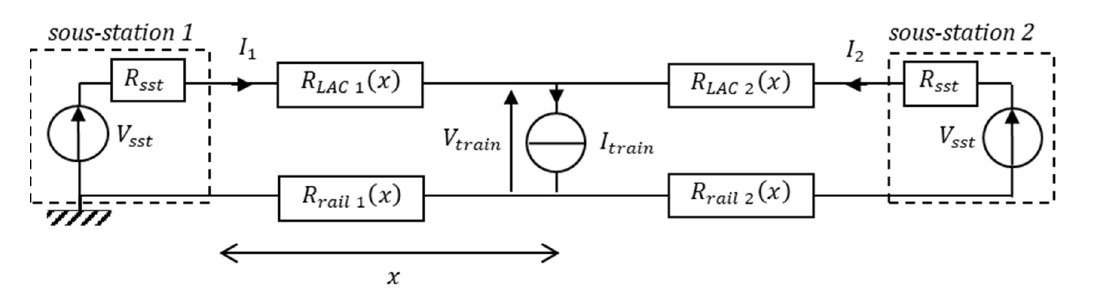
\includegraphics[width=0.75\textwidth]{Figures/Schematic.png}
            \caption{Schéma du modèle.}
            \label{fig:Schematic}
        \end{figure}

    \section*{La fonction \texttt{Simulation()}}\addcontentsline{toc}{section}{La fonction \texttt{Simulation()}}
        \subsection*{Sans Batterie}\addcontentsline{toc}{subsection}{Sans Batterie}
            Lors de l’analyse du mouvement du train, les graphiques montrent les interactions entre la
            position, la vitesse et l’accélération. Une phase d’accélération entraîne une augmentation plus
            marquée des courbes de position et de vitesse. À l’inverse, pendant le freinage, la position évolue
            lentement tandis que la vitesse et l’accélération diminuent progressivement jusqu’à atteindre zéro,
            tant que l’accélération reste nulle.

            \begin{figure}[H]
                \centering
                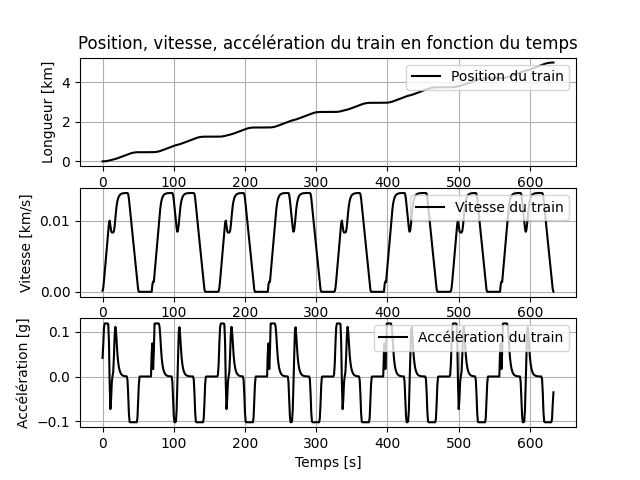
\includegraphics[width=0.75\textwidth]{Figures/xvf.png}
                \caption{Position, Vitesse et Accélération du train.}
                \label{fig:xvf}
            \end{figure}

            Pour calculer ces variations, la fonction
            np.gradient a été utilisée.

            Ensuite, la puissance du train a été déterminée en intégrant les forces résistives, motrices et
            mécaniques, en tenant compte d’un rendement global de $80$\%{} pour la chaîne de conversion.

            \begin{figure}[H]
                \centering
                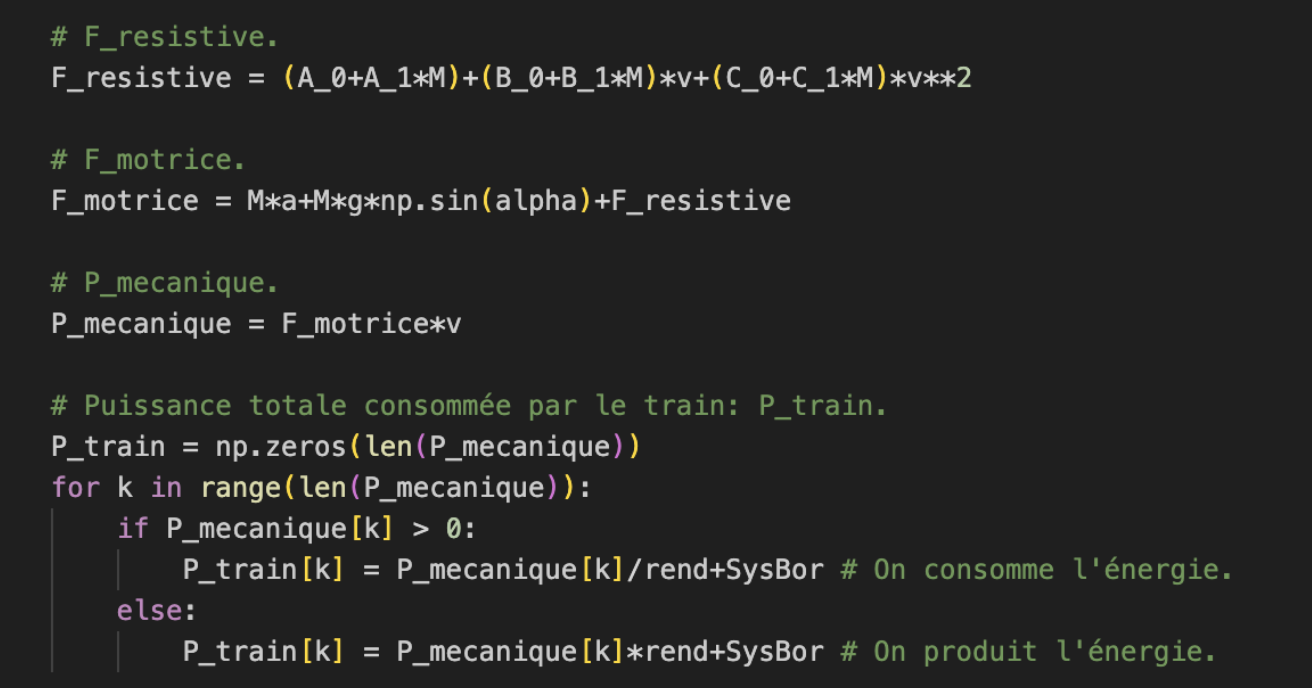
\includegraphics[width=0.75\textwidth]{Figures/AdamCode_0.png}
                \caption{}
                \label{fig:AdamCode_0}
            \end{figure}

        \subsection*{Avec Batterie}\addcontentsline{toc}{subsection}{Avec Batterie}
            L’introduction d’une batterie (rendement de $90$\%{}, capacité de $10$ kWh et tension de seuil de $400$~kV) modifie les dynamiques observées. Les graphiques indiquent que les relations entre la
            puissance, la tension et le courant restent cohérentes. Durant les phases d’accélération, la
            batterie se décharge, tandis qu’elle se recharge lors du freinage. Grâce à sa grande capacité et à
            sa tension élevée, la batterie ne se décharge jamais complètement.

            Concernant la gestion de la batterie, on a suivit la logique (indiqué figure \ref{fig:AdamCode_1}):

            \begin{figure}[H]
                \centering
                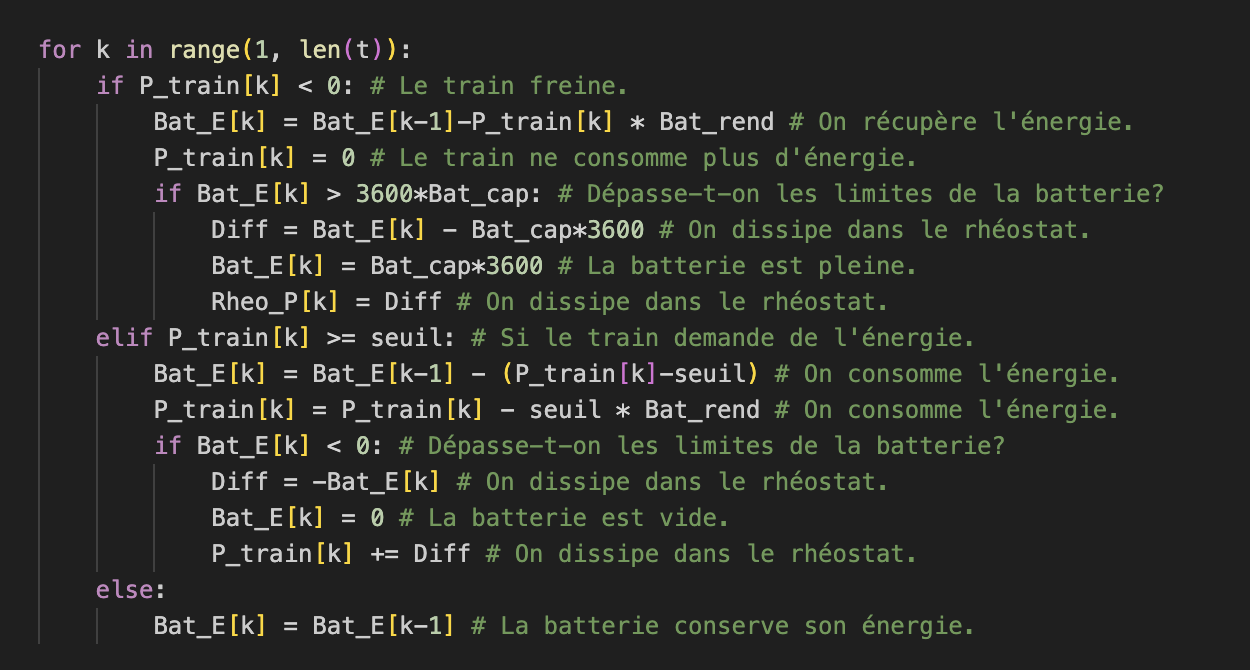
\includegraphics[width=0.75\textwidth]{Figures/AdamCode_1.png}
                \caption{Gestion de la batterie.}
                \label{fig:AdamCode_1}
            \end{figure}

            Le système globale peut-être schématiser comme le modèle ci-dessous:

            \begin{figure}[H]
                \centering
                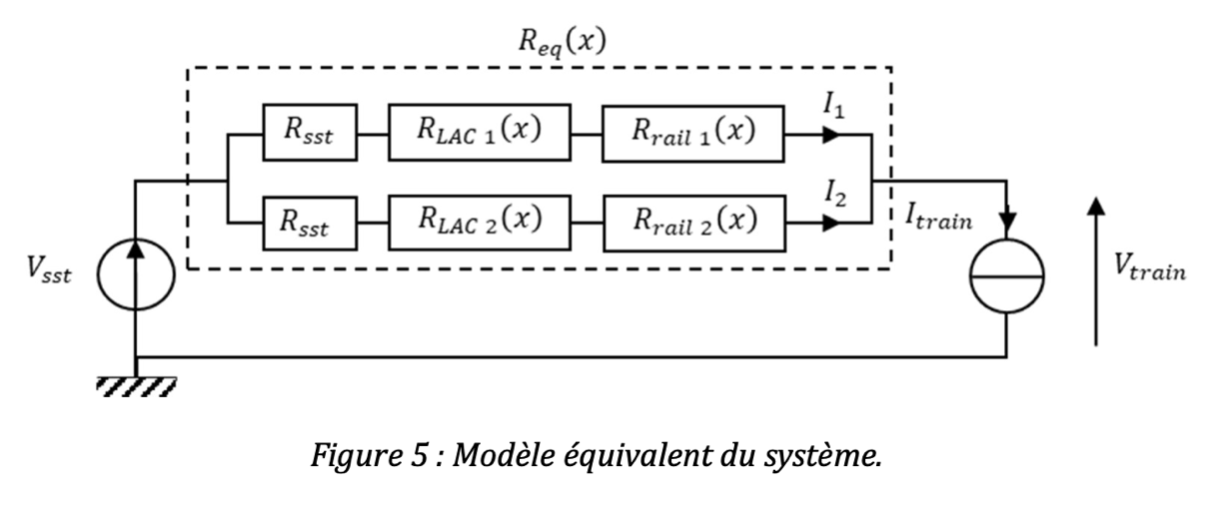
\includegraphics[width=0.75\textwidth]{Figures/AdamCode_2.png}
                \caption{Schéma des résistances du circuit.}
                \label{fig:AdamCode_2}
            \end{figure}

            \begin{gather*}
                R_{\text{LAC1}} = \rho_{\text{LAC}} x\\
                R_{\text{LAC2}} = \rho_{\text{LAC}} \left(x_{\text{Tot}}-x\right)\\
                R_\text{rail1} = x\rho_\text{rail}\\
                R_\text{rail2} = \left(x_\text{Tot}-x\right)\rho_\text{rail}\\
                R_\text{eq} = \frac{\left(R_\text{SST}+R_\text{LAC1}+R_\text{rail1}\right)\left(R_\text{SST}+R_\text{LAC2}+R_\text{rail2}\right)}{2R_\text{SST}+R_\text{LAC1}+R_\text{LAC2}+R_\text{rail1}+R_\text{rail2}}
            \end{gather*}

            Cela nous permet ainsi de calculer la tension et le courant du train.

            \begin{figure}[H]
                \centering
                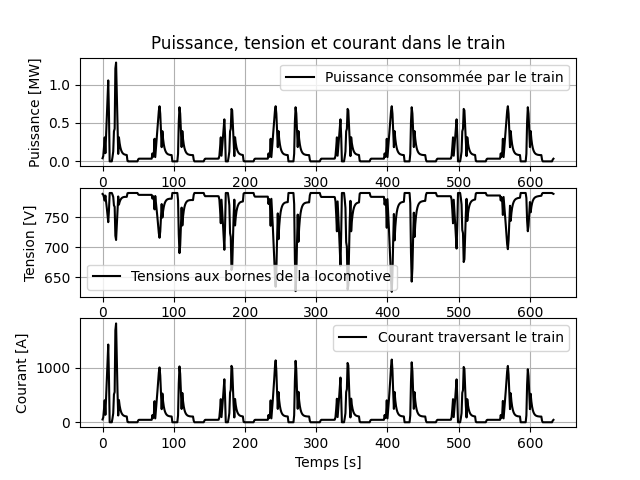
\includegraphics[width=0.75\textwidth]{Figures/PTI.png}
                \caption{Puissance, tension et courant du train.}
                \label{fig:PTI}
            \end{figure}

            On observe ainsi que les relations entre la puissance, la tension et le courant sont respecté. Lors
            des phases d’accélération ou de freinage on a une variation de ces éléments.

            Concernant la batterie, celle ci réagit également comme nous l’avions prévu, à savoir que lors du
            freinage celle-ci se recharge, puis lors des phases d’accélération elle se décharge. Étant donné
            que nous avons prit une très grande batterie ($10$~kW) et une tension de seuil élevé, la batterie ne se
            décharge jamais complètement.

            \begin{figure}[H]
                \centering
                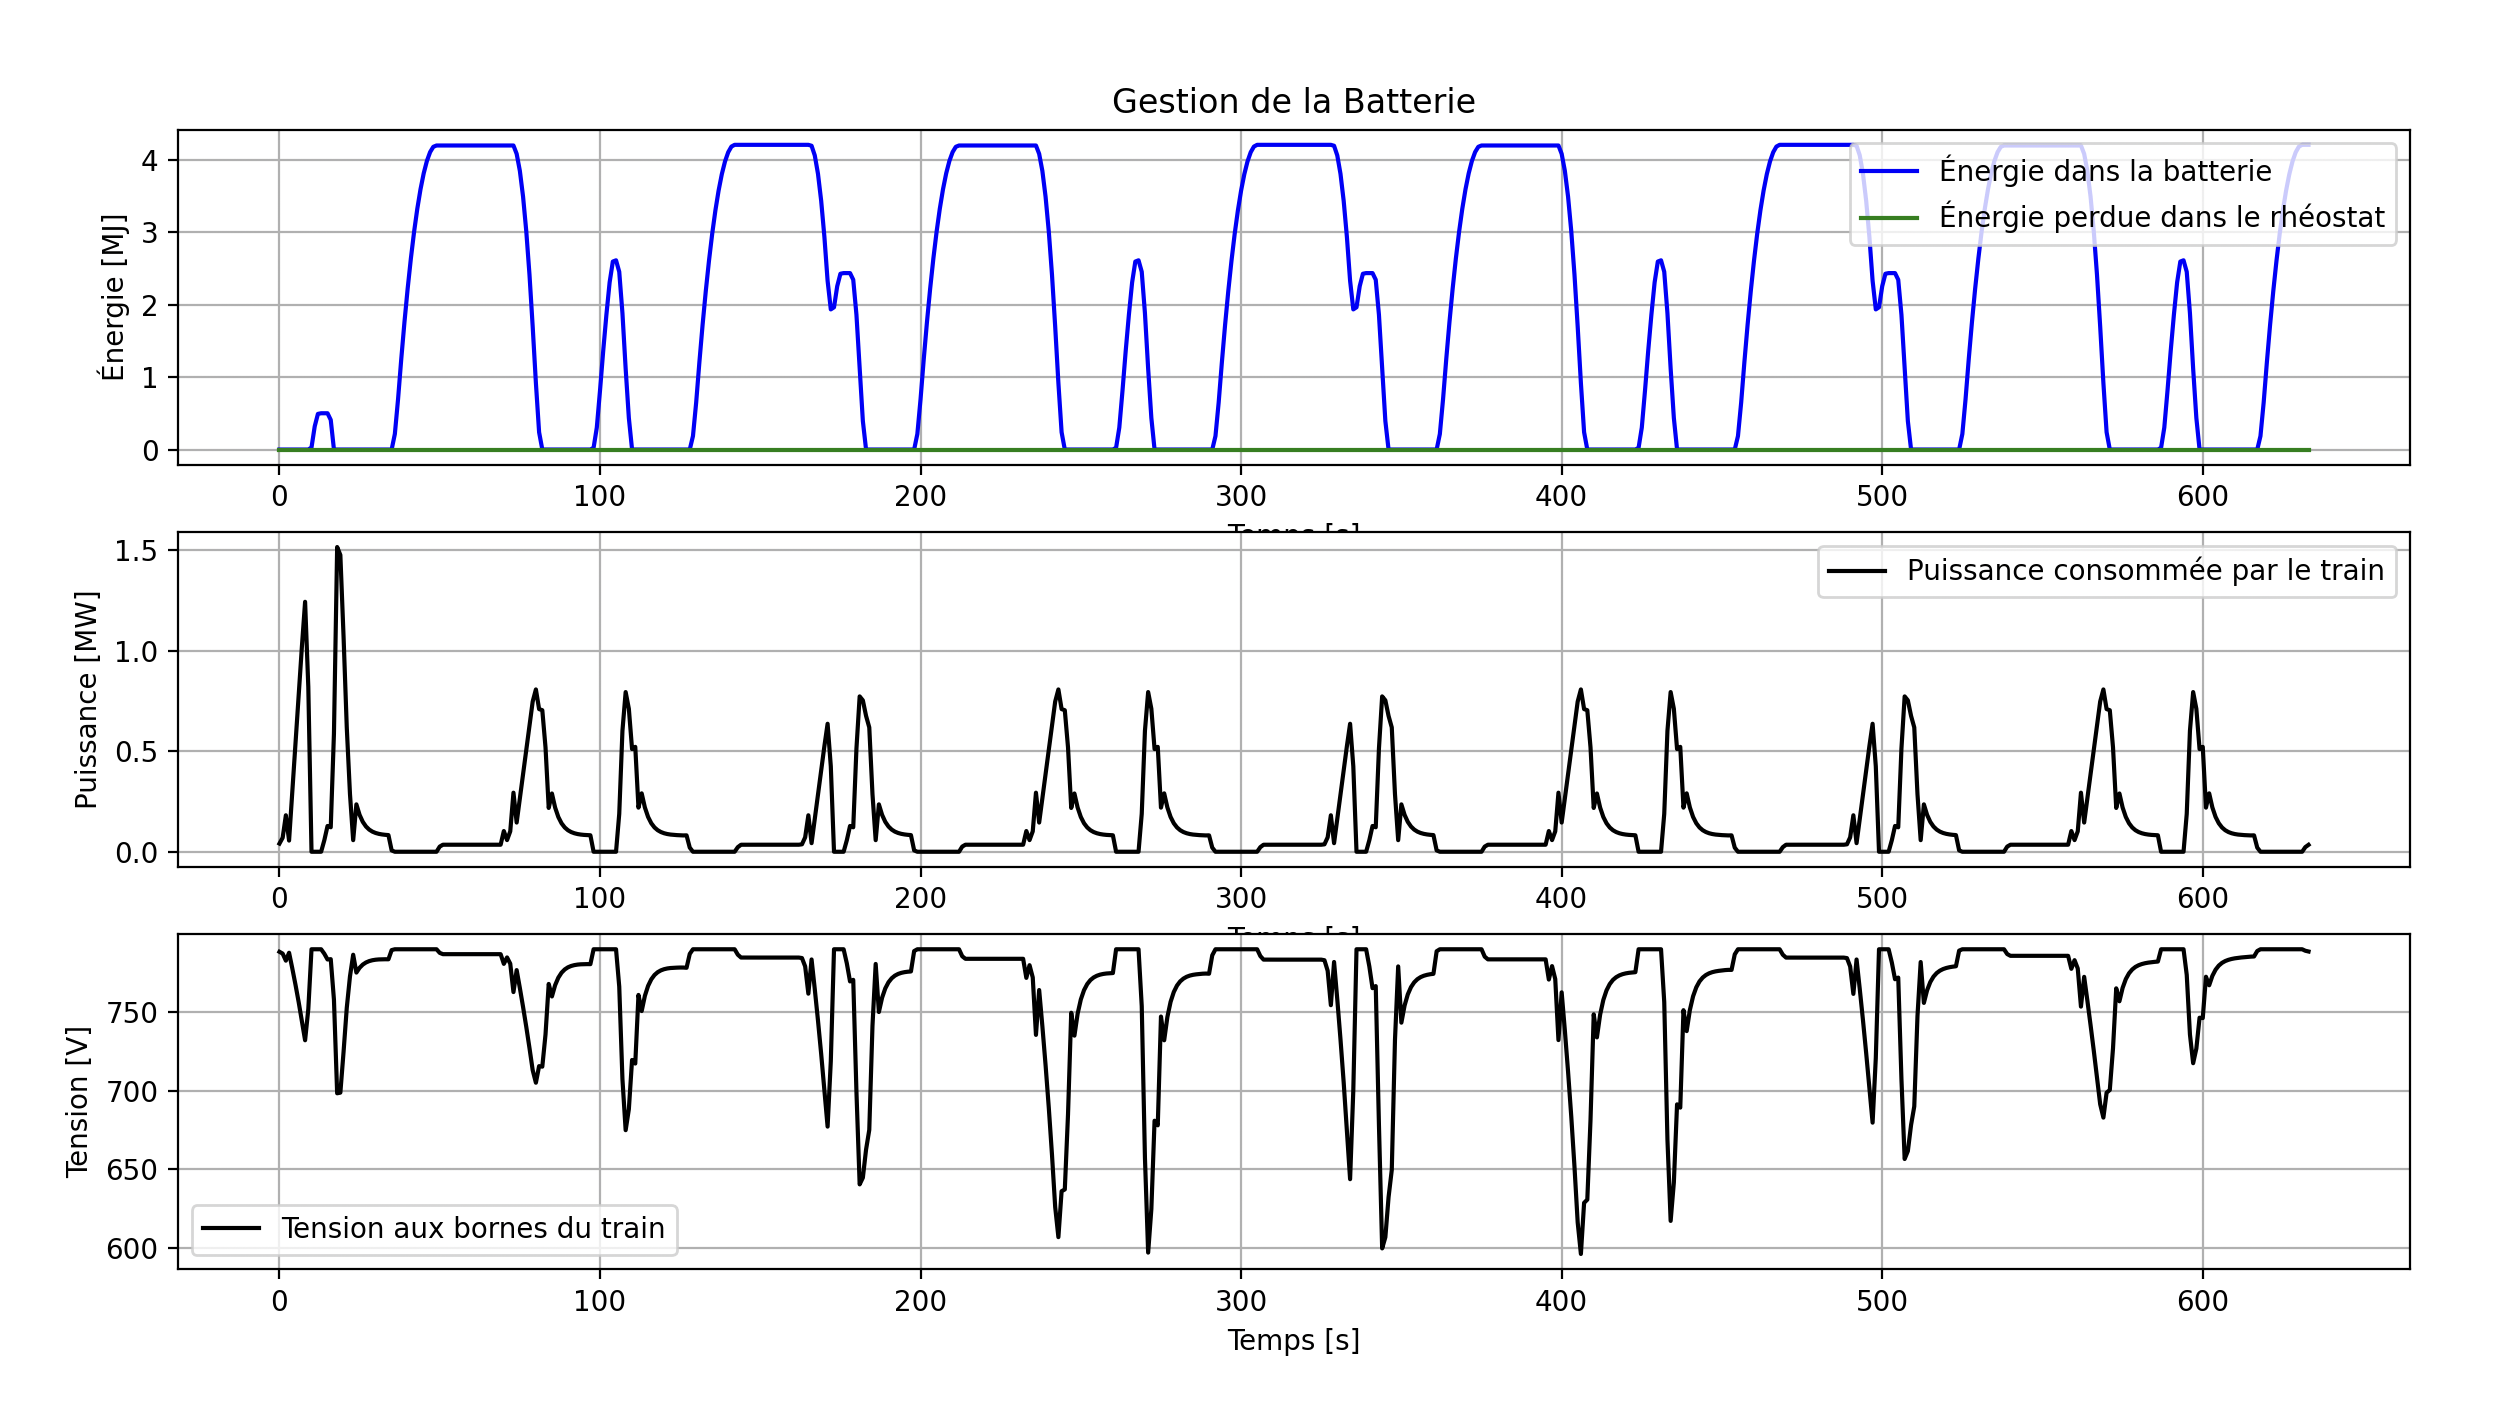
\includegraphics[width=0.75\textwidth]{Figures/Bat.png}
                \caption{Gestion de la batterie.}
                \label{fig:Bat}
            \end{figure}

            \subsection*{Analyse des sous-stations et qualité du système}\addcontentsline{toc}{subsection}{Analyse des sous-stations et qualité du système}
            Les graphiques montrent que le courant et la puissance dans les LAC (Lignes Aériennes de
            Contact) des sous-stations sont équilibrés. On constate également que, lorsque le train
            s’approche de la sous-station 2, la puissance et le courant fournis par celle-ci augmentent
            proportionnellement.

            \begin{figure}[H]
                \centering
                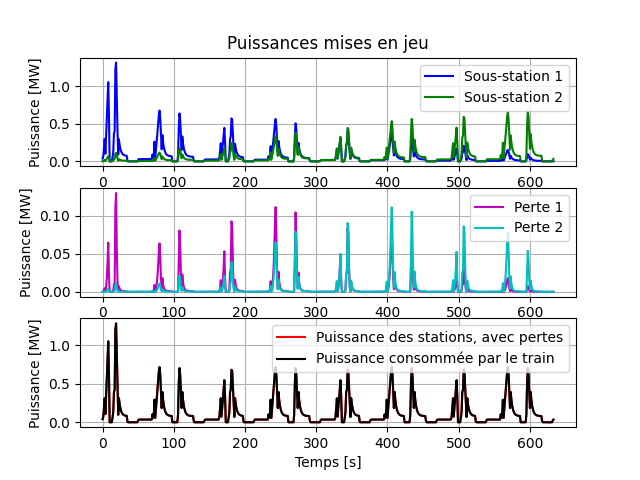
\includegraphics[width=0.75\textwidth]{Figures/P.png}
                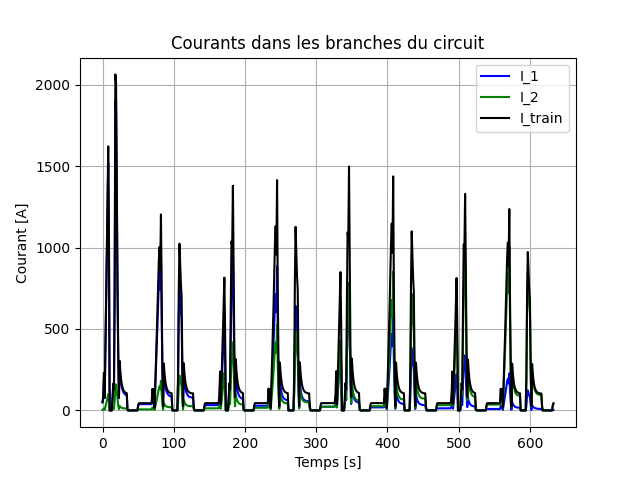
\includegraphics[width=0.75\textwidth]{Figures/I.png}
                \caption{Puissances et courants mis en jeu.}
                \label{fig:PI}
            \end{figure}

            Un indicateur clé de performance, la chute de tension maximale, est utilisé pour évaluer la qualité
            du système. Cet indicateur pourrait être optimisé en choisissant une batterie et une tension de
            seuil mieux adaptées.

            \begin{figure}[H]
                \centering
                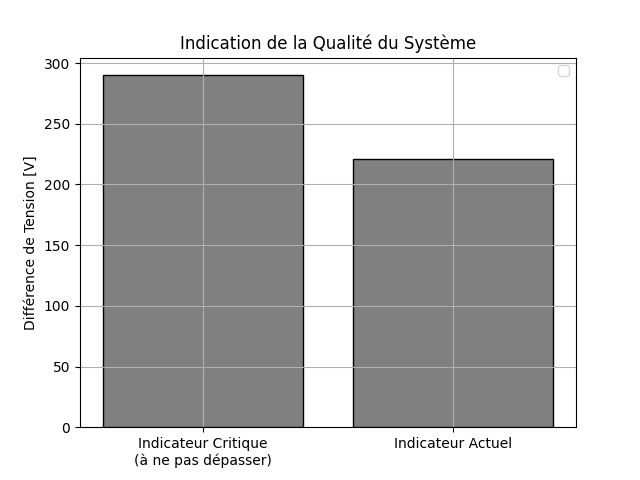
\includegraphics[width=0.75\textwidth]{Figures/Qual.png}
                \caption{Chute de tension (indicateur de qualité) du système.}
                \label{fig:Qual}
            \end{figure}

    \section*{Monte-Carlo}\addcontentsline{toc}{section}{Monte-Carlo}


    \section*{Algorithme NSGA-II}\addcontentsline{toc}{section}{Algorithme NSGA-II}
        L'algorithme génétique NSGA-II (\emph{Non-Dominated Sorting Generic Algorithm 2}) permet de trouver les meilleures solutions dans un contexte donné de façon assez efficace.
        Cet algorithme génère une population de taille $N$ d'individus (les solutions), puis recherche au sein de cette population les \guillemotleft{}~solutions non-dominées~\guillemotright{}, et les range en suivant cette ordre:

        ---~En premier, les solutions non-dominées, c'est-à-dire celles qui dominent toutes le autres, les meilleures de la population.

        ---~En deuxième, les solutions non-dominées qui restent, en ayant retirées les solutions précédentes de la population de départ.

        ---~ En troisième, les solutions non-dominées restantes, en ayant retirées toutes les précédentes de la population de départ.

        ---~On continue jusqu'à épuisement des individus dans la population de départ.

        Ayant maintenant à notre diposition un classement des individus selon leurs performances, on sélectionne les $50\%{}$ meilleurs dans ce classement, puis les croisons afin de créer la génération suivante.
        Puis le cycle recommence, pour un total de $N$ itérations.

        Il faut savoir que NSGA-II, demandant un classement des solutions selon leur dominance, doit utiliser une fonction qui classe les solutions selon cette ordre. Pour ceux qui regarderaient notre code, il s'agit de la fonction \texttt{non\_dominant\_sort()} (voir figure \ref{fig:non_dominant_sort}).

        \begin{figure}[H]
            \centering
            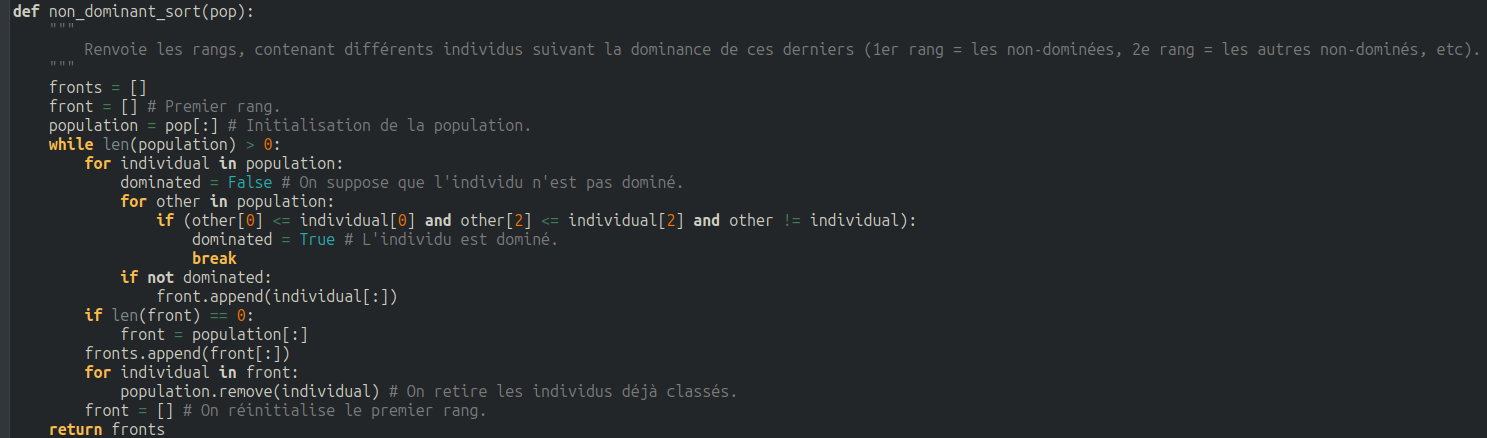
\includegraphics[width=\textwidth]{Figures/non_dominant_sort.png}
            \caption{Code de la fonction du classement en fronts.}
            \label{fig:non_dominant_sort}
        \end{figure}

        Et, pour sélectionner les $50\%{}$ meilleurs, nous utilisons la fonction ci-dessous affichée en figure \ref{fig:select_half_best}:

        \begin{figure}[H]
            \centering
            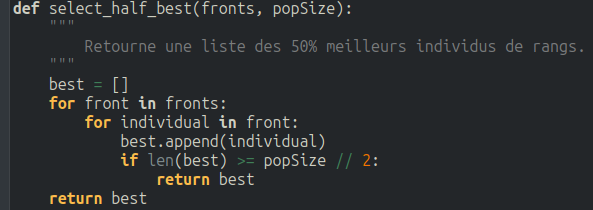
\includegraphics[width=0.75\textwidth]{Figures/select_half_best.png}
            \caption{Sélection des $50\%{}$ meilleurs.}
            \label{fig:select_half_best}
        \end{figure}

        Comme affiché sur la figure \ref{fig:NSGA2}, les solutions intéressantes pour notre batterie semblent se trouver aux alentours de $1,5$ ou $2$~kWh, pour un seuil vers les $300$~kW et une chute de $200$~V (les points rouges représentant la dernière génération créée par notre algorithme).
        Suivant la simulation, les résultats peuvent énormément changer, et il est conseiller de relancer plusieurs fois l'algorithme afin de trouver des solutions potentiellement meilleures.
        Par ailleurs, étant donné l'absence de \guillemotleft{}~\emph{crowding\_distance}~\guillemotright{}, nommé \guillemotleft{}~critère de distance~\guillemotright{} en français, nos solutions tendent à se rassembler en un amas compact; augmenter le taux de mutation peut sensiblement améliorer ce problème.

        \begin{figure}[H]
            \centering
            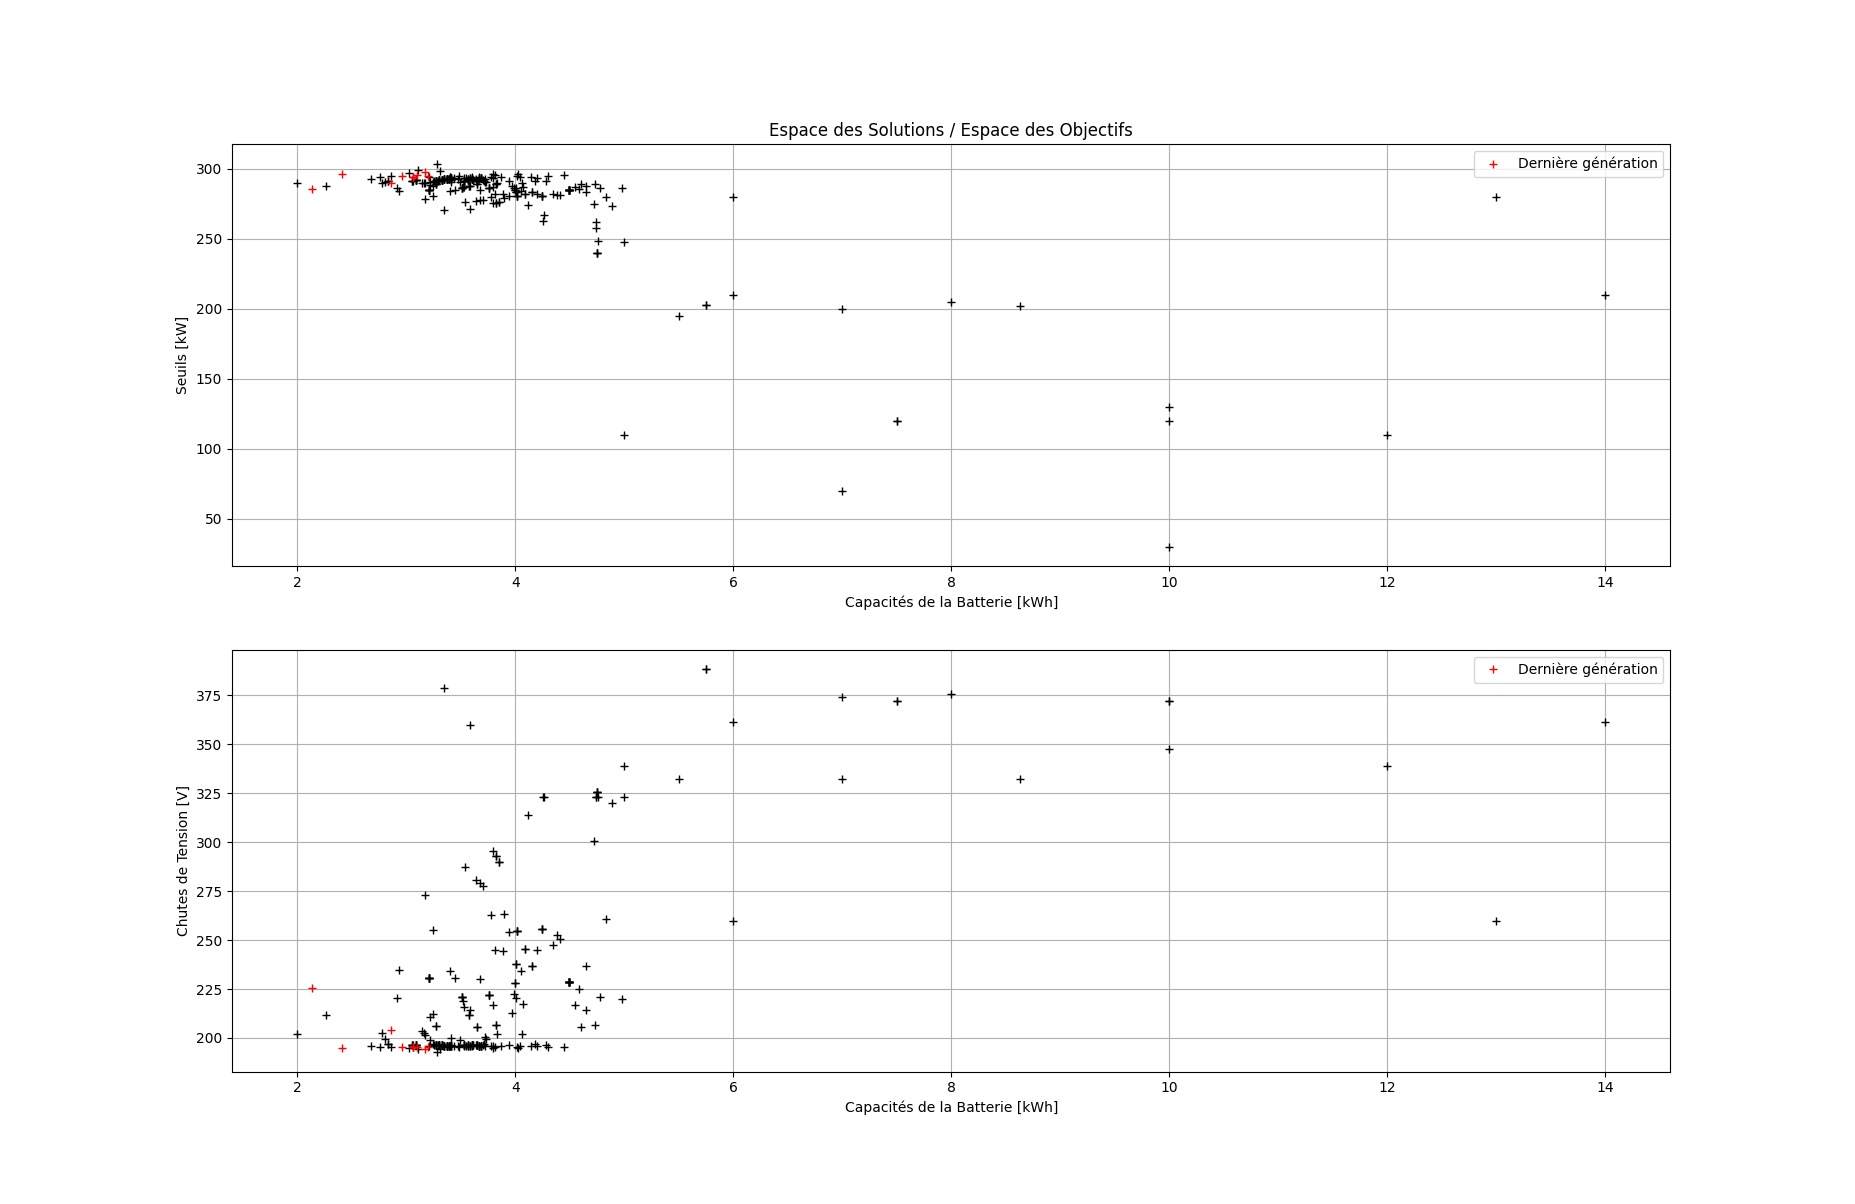
\includegraphics[width=0.75\textwidth]{Figures/NSGA-II.png}
            \caption{Résultats de l'algorithme NSGA-II.}
            \label{fig:NSGA2}
        \end{figure}


    \section*{Conclusion}\addcontentsline{toc}{section}{Conclusion}
        Pour conclure, nous pouvons dire que l'algorithme NSGA-II est plus efficace que la méthode Monte-Carlo; en revanche, Monte-Carlo s'étend dès le départ sur un maximum de résultats, là où NSGA-II (en particulier notre version simplfifée) peut rester coincé à quelques valeurs seulement (d'où l'intérêt d'avoir une population suffisamment large, et un taux de mutation pas trop bas, mais trop haut non plus).

        Comme résultat final, nous pouvons mettre en avant une batterie de capacité $1,5$~kWh et un seuil de $300$~kW auquel le train commence à demander de l'énergie à la batterie.
        Les résultats sont donnés en figure \ref{fig:Con}, pour de tels paramètres.

        \begin{figure}[H]
            \centering
            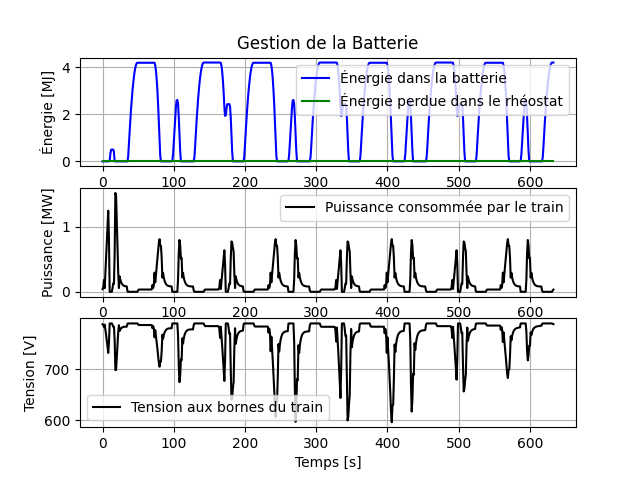
\includegraphics[width=0.75\textwidth]{Figures/Bat_F.png}
            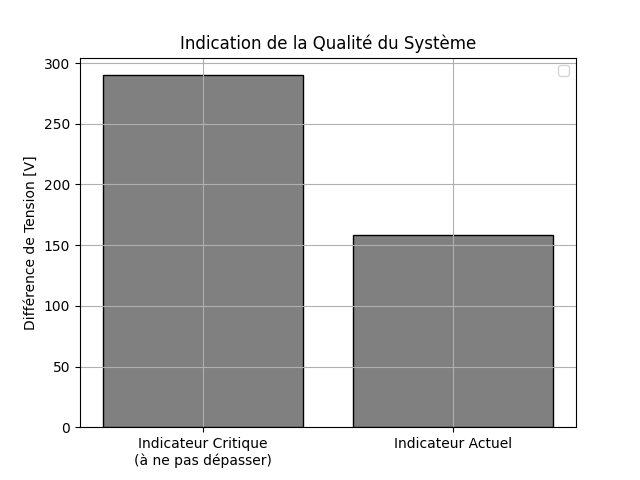
\includegraphics[width=0.75\textwidth]{Figures/Qual_F.png}
            \caption{Résultats de la simulation du train, pour une batterie de capacité $1,5$~kWh et un seuil de $300$~kW (paramètres optimisés selon l'algorithme NSGA-II). L'indicateur de qualité est représenté par la chute de tension maximale aux bornes du train; une chute de plus de $290$~V est dangereuse.}
            \label{fig:Con}
        \end{figure}

        Évidemment, d'autres batteries avec seuil optimisés sont également disponibles (revoir figure \ref{fig:NSGA2}).

\end{document}

% Simulation(10000, 400000, True)
